% TODO: Update these numbers when we are given new datasets.
\section{Data} \label{sec:data}

As described earlier we use data from the Danish company MaCom. The dataset
provided by MaCom is a file consisting of set of texts in Danish where each text
is associated with an author ID. We have been given several text extractions
of different sizes with the biggest dataset consisting of 32,682 texts. The
dataset consist of texts of many different sizes. The shortest text consist of 2
characters and the longest text of 1.849.919 characters. The average length of
each text is 5689 characters with a median of 5363 characters. That means that
almost all texts is close to the average and only a few has sizes much greater
or smaller than the average. The dataset contains 2047 different authors with
an average of 16 texts. The author with the smallest amount of text has two
texts and the author with the most amount of text has 33 texts.

In several of our experiments we limited the number of different characters
we represented. We did that to simplify the amount of different characters
our neural networks had to consider. In particular we cutoff any characters
that occurred with a frequency less than $\frac{1}{100,000}$. We wanted to
make sure that the cutoff only removed characters that were so infrequent
that it would be hard for the neural networks to learn anything from them.
Since the average amount of characters in a single text were 5851 characters
most texts wont include any character that has a frequency below the above
cutoff point. While we wanted to limit the number of different characters
the network would have to consider we also wanted to make sure that a couple
of Danish characters would be considered. In particular the characters \ae,
\o, \aa, \AE, \O\ and \AA. Those characters occur with the frequencies
$7.23\cdot10^{-3}$, $5.5\cdot10^{-3}$, $8.5\cdot10^{-1}$, $1.85\cdot10^{10-5}$,
$3.13\cdot10^{-5}$ and $2.08\cdot10^{-5}$ respectively and will therefore
all be included. The overall frequency distribution can be seen in figure
\ref{fig:character_frequencies}.

\begin{figure}[htb]
    \centering
    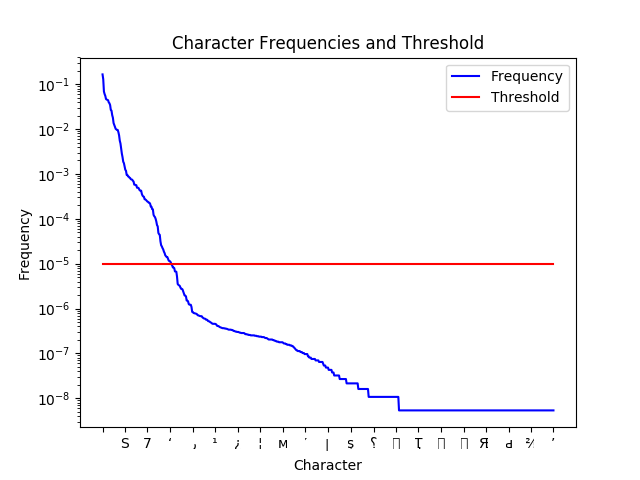
\includegraphics[scale=.8]{./graphs/data/character_frequencies.png}
    \caption{The frequency distribution of characters in the training data-set,
        only a random subset of characters is shown on the x-axis, including the
        most and least frequent}
    \label{fig:character_frequencies}
\end{figure}

% TODO: Describe how we dealt with garbage texts.
The texts we are given are extracted from \textit{.pdf} files and there will
therefore sometimes be garbage included.
